\documentclass{VUMIFPSkursinis}
\usepackage{algorithmicx}
\usepackage{algorithm}
\usepackage{algpseudocode}
\usepackage{amsfonts}
\usepackage{amsmath}
\usepackage{bm}
\usepackage{caption}
\usepackage{color}
\usepackage{float}
\usepackage{graphicx}
\usepackage{listings}
\usepackage{float}
\usepackage{subfig}
\usepackage{wrapfig}
\usepackage[hidelinks]{hyperref}
\usepackage{todonotes}
\usepackage{xcolor}
\usepackage{lineno}
\linenumbers
% Titulinio aprašas
\university{Vilniaus universitetas}
\faculty{Matematikos ir informatikos fakultetas}
\department{Programų sistemų katedra}
\papertype{Programų kūrimo proceso laboratorinis darbas}
\title{Įmonės ,,Mėnuliukų technologijos" programų kūrimo proceso aprašas}
\titleineng{Description of the development process of the ,,Mėnuliukų technologijos" company}
\status{4 kurso 3 grupės studentai}
\author{Mėnuliukai}


\supervisor{Saulius Ragaišis, Doc., Dr.}
\date{Vilnius – \the\year}

% Nustatymai
% \setmainfont{Palemonas}   % Pakeisti teksto šriftą į Palemonas (turi būti įdiegtas sistemoje)
\bibliography{bibliografija}

\begin{document}
\maketitle

\tableofcontents

\sectionnonum{Įvadas}
	\textcolor{green}{Šiame darbe bus pristatytas ,,Mėnuliukų technologijų" programų kūrimo procesas.}
	Pats procesas yra paremtas Agile metodologija su minimaliais pakeitimais reikalavimų rinkime.
	Proceso pradžioje stengiamės su užsakovu išsiaiškinti norimus įgyvendinti funkcionalumus ir bendraujant kartu su užsakovu sudaryti reikalavimus.
	Sudarant reikalavimus yra diskutuojama ir sistemos ateities vizija, siekiant susidaryti geresnę perspektyvą sistemos ateičiai ir darbartiniams reikalavimams.
	Įmonė įvertina, kiek valandų užtruks kiekvieno funkcionalumo sukūrimas, o mokestis yra imamas už pradirbtas valandas.
	Klientui nesutikus su pateiktomis kainomis yra daromi susitikimai siekiant paaiškinti valandų vertinimą. Po susitikimų funkcionalumo įgyvendinimo valandos gali keistis, arba funkcionalumas bus atsisakytas.
	Kiekvieno sprinto pradžioje, po reikalavimų pasitikslinimo, yra sudaromi priėmimo testai, kuriuos praėjus kliento prašoma susimokėti už atliktus darbus.

\section{Kūrimo procesas}
	\begin{figure}[htbp]
		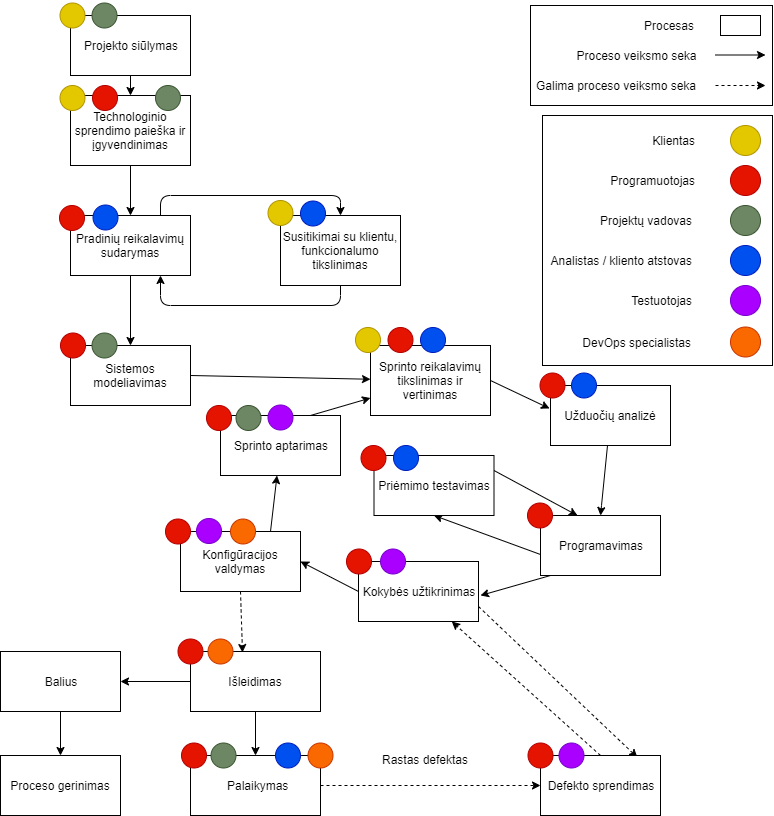
\includegraphics[scale=0.6]{img/SoftwareProcessMoonTechnologies}
		\caption{Sistemos kūrimo procesas} % Antraštė įterpiama po paveikslėlio
		\label{img:kurimoProcesas}
	\end{figure}

	\newpage

	\subsection{Projekto siūlymas}
	\begin{center}
		\begin{table}[ht]
			\caption{Projekto siūlymo procesas}
			\begin{tabular}{ | l | l | }
				\hline
				Pavadinimas:          & Projekto siūlymas.						\\ \hline
				Tikslas:              & \textcolor{green}{Aptarti galimą projektą su galimu klientu.}			\\ \hline
				Vykdytojai:           & \textcolor{green}{Projekto vadovas ir klientas.}					\\ \hline
				Veiklos:              & \textcolor{green}{V1 - Aptariama sistemos aprėptis. }				\\
				                      & \textcolor{green}{V2 - Nustatomos kainos ribos iki pirmo sistemos išleidimo.}	\\
				                      & \textcolor{green}{V3 - Pirminės sutarties pasirašymas.}				\\ \hline
				Naudojami produktai:	& \textcolor{green}{NP1 - Buvusių projektų dokumentai. }				\\ \hline
				Sukuriami produktai:	& \textcolor{green}{SP1 - Pirminė sutartis sistemos projektavimui.	}	\\ \hline
			\end{tabular}
		\end{table}
	\end{center}

	\begin{enumerate}
		\item{
			Pirmas susitikimas, kuriame aptariamas galimas projektas, kiekviena pusė išsako savo lūkesčius, pasidalinama idėjomis.
		}
		\item{
			Po susitikimo įmonė paruošia pradinį pasiūlymą, į kurį įeina orientacinės finansų ribos, žmonių ištekliai, kurie galėtų būtų skiriami šiam projektui.
			Šis pasiūlymas aptariamas su klientu, kartu su juo dokumentuojami funkcionalumai, kurių klientas nori pirmame sistemos išleidime.
			Sėkmingai tęsiantis tolesnėms deryboms nutariama dėl pradinio technologinio sprendimo pasiūlymo datos bei finansavimo jam.
		}
		\item{
			Pasirašoma pradinė sutartis, kurioje dokumentuojama prieš tai aptarta informacija.
			Ši sutartis galioja iki pirmojo prototipo pasiūlymo, po kurio atnaujinamos derybos dėl tolesnio projekto vystymosi.
		}
	\end{enumerate}

	\subsection{\textcolor{green}{Technologinio sprendimo paieška ir įgyvendinimas}}
	\begin{center}
		\begin{table}[ht]
			\caption{Technologinio sprendimo paieškos ir įgyvendinimo procesas.}
			\begin{tabular}{ | l | l | }
				\hline
				Pavadinimas:          & Technologinio sprendimo paieška ir įgyvendinimas.									\\ \hline
				Tikslas:              & \textcolor{green}{Išskirti technologijas ir jų versijas, kurios bus naudojamos projekte. 	}					\\ \hline
				Vykdytojai:           & \textcolor{green}{Projekto vadovas, klientas, programuotojas.}										\\ \hline
				Veiklos:              & \textcolor{green}{V1 - Aptarti technologijas, šiuo metu naudojamas projekte.} 								\\
				                      & \textcolor{green}{V2 - Nustatomos technologijų kainos, kurios bus naudojamos projekte.}							\\
				                      & \textcolor{green}{V3 - Nutariama dėl technologinių alternatyvų.	}									\\ \hline
				Naudojami produktai:	& \textcolor{green}{NP1 - Esamos sistemos dokumentacija, norimų naudoti technologijų} \\& \textcolor{green}{dokumentacija ir kainynas. 	}		\\ \hline
				Sukuriami produktai:	& \textcolor{green}{SP1 - Technologinių sprendimų ir jų alternatyvų dokumentas su} \\& \textcolor{green}{preliminariomis technologijų licenzijų kainomis.}	\\ \hline
			\end{tabular}
		\end{table}
	\end{center}
	\newpage
	\begin{enumerate}
		\item{
			Aptariamos technologijos, kurios šiuo metu naudojamos projekte - išskiriami technologiniai karkasai, duomenų bazės, programavimo kalbų versijos ir kitos naudojamos technologijos ir jų versijos.
			Įvertinamas esamų technologijų saugumo lygis, greitaveika ir ateities palaikymas.
			Pasiūlomi technologiniai sprendimai pagrindžiant jų naudą sistemai.
		}
		\item{Nustatomos technologijų kainos, kurios bus naudojamos projekte - paskaičiuojamos dabartinių technologijų kainos ir naujų siūlomų technologijų kainos.}
		\item{
			Nutariama dėl technologinių alternatyvų - jeigu įmanoma klientui pasiūlomi atviro kodo technologiniai sprendimai siekiant sutaupyti pinigų.
			Pateikiamas palyginimas tarp dabartinės sistemos technologijos, siūlomos technologijos ir atviro kodo technologijų sprendimų.
		}
	\end{enumerate}

	\subsection{Reikalavimų ciklas}
	\begin{center}
		\begin{table}[ht]
			\caption{Reikalavimų ciklo procesas.}
			\begin{tabular}{ | l | l | }
				\hline
				Pavadinimas:          & Reikalavimų ciklas.                                                                                                            \\ \hline
				Tikslas:              & \textcolor{green}{Suformuoti funkcinius ir nefunkcinius reikalavimus.}                                                         \\ \hline
				Vykdytojai:           & \textcolor{green}{Programuotojas, analistas, klientas.}                                                                        \\ \hline
				Veiklos:              & \textcolor{green}{V1 - Iš kliento pateiktų verslo reikalavimų suformuojame funkcinius} \\& \textcolor{green}{reikalavimus.}    \\
															& \textcolor{green}{V2 - Pristatome klientui sudarytus funkcinius reikalavimus ir tiksliname} \\& \textcolor{green}{pateiktus verslo reikalavimus.} \\
				                      & \textcolor{green}{V3 - Siūlomi nefunkciniai reikalavimai.}                                                                     \\ \hline
				Naudojami produktai:  & \textcolor{green}{NP1 - Kliento pateiktas verslo reikalavimų dokumentas.}                                                      \\ \hline
				Sukuriami produktai:  & \textcolor{green}{SP1 - Funkcinių ir nefunkcinių reikalavimų dokumentas.}                                                      \\ \hline
				                      & \textcolor{green}{SP2 - Susaistytų šalių parašai reikalavimam patvirtinti.}                                                    \\ \hline
			\end{tabular}
		\end{table}
	\end{center}

	\begin{enumerate}
		\item{
			\textcolor{green}{Iš užsakovo ir naudotojų pateiktų verslo reikalavimų suformuojame funkcinius ir nefunkcinius reikalavimus.
			Su visom partijom, įskaitant užsakovus ir naudotojus, susėdama, aptariami reikalavimai ir taip suderinami, kad visos susaistytos šalys būtų patenkintos.
			Iš visų partijų surenkami parašai, tam kad vėliau nekiltų klausimų, kodėl reikalavimai neatitinka įsivaizdavimų.
			Mūsų įmonės verslo analitikas dirbdamas kartu su programuotojais suformuoja atsekamus (su indentifikacijos kodu) funkcinius ir nefunkcinius} reikalavimus.
		}
		\item{
			\textcolor{green}{Kompanija pateikia prieigą prie sistemos, su visu reikalavimų sąrašu, kur užsakovai gali stebėti jų įvykdymą.}
			Testuojant suprogramuotą funkcionalumą ir įgyvendinus reikalavimą, sistemoje pažymimas jog reikalavimas įgyvendintas.
		}
		\item{
			\textcolor{green}{Išsiaiškinami baziniai reikalavimai, kurie yra patys svarbiausi ir turi būti pirmi igyvendinti, baziniai reikalavimai yra atitinkamai pažymimi sistemoje.
			Baziniai reikalavimai yra ypač atidžiai analizuojami analistų, analizėje taip pat įvertinama, kokia tikimybė, jog pasikeis reikalavimas ir atitinkamai suplanuojami veiksmai tokiu atveju.}
		}
		\item{
				\textcolor{green}{Pristatome klientui sudarytus funkcinius reikalavimus ir tiksliname pateiktus verslo reikalavimus - suformavus funkcinius reikalavimus planuojami susitikimai su klientu, siekiant jam pristatyti suformuotus reikalavimus, patikslinti pateiktus verslo reikalavimus ir toliau tikslinti reikalavimus iki kol reikalavimai tenkins klientą ir bus suprantami programuotojų komandai, kuri dirbs prie kliento projekto.}
		}
		\item{
			\textcolor{green}{Siūlomi nefunkciniai reikalavimai - jeigu klientas pats nepateikė nefunkcinių reikalavimų įmonė pati pateikia nefunkcinių reikalavimų siūlymus pagal esamo projekto apimtį ir biudžetą.
			Pateikti nefunkciniai reikalavimai yra aptariami ir tikslinami su klientu.}
		}
		\item{
			\textcolor{green}{Jeigu klientas reikalavimą pakeičia programavimo fazėje tai reikalavimas yra atidžiai peržiūrimas dar kartą, įvertinama, kiek kitokio funkcionalumo reikės pakeisti kuriamoj programų sistemoje, ir klientui pateikiama nauja sutartis, kurioje aprašoma, kokie darbai bus atlikti tam, kad jau suprogramuotoje sistemoje pakeistas reikalavimas būtų įgyvendintas.
			Dar neįgyvendintų reikalavimų keitimas yra pigesnis (nes nereikia perprogramuoti nieko) ir klientui aiškiai išdėstoma kainos struktūra, kiek nauja sutartis kainuos, jeigu būs keičiami reikalavimai, kurie jau įgyvendinti.}
		}
	\end{enumerate}

	\newpage

	\subsection{Sistemos modeliavimas}
	\begin{center}
		\begin{table}[ht]
			\caption{Sistemos modeliavimo procesas}
			\begin{tabular}{ | l | l | }
				\hline
				Pavadinimas:         & Sistemos modeliavimas.                                                \\ \hline
				Tikslas:             & \textcolor{green}{Sukurti pradinę sistemos versiją.}                  \\ \hline
				Vykdytojai:          & \textcolor{green}{Programuotojas, analistas.}                         \\ \hline
				Veiklos:             & \textcolor{green}{V1 - Reikalavimų analizė iš implementacijos pusės.} \\
				                     & \textcolor{green}{V2 - Pradinės sistemos rašymas ir testavimas.}      \\
				                     & \textcolor{green}{V3 - Atnaujintos sutarties pasirašymas.}            \\ \hline
				Naudojami produktai: & \textcolor{green}{NP1 - Sistemos reikalavimai.}                       \\
				                     & \textcolor{green}{NP2 - Architektūrinių sprendimų dokumentas.}        \\ \hline
				Sukuriami produktai: & \textcolor{green}{SP1 - Pradinė kodo bazė.}                           \\ \hline
			\end{tabular}
		\end{table}
	\end{center}

	\begin{enumerate}
		\item Pagal gautus reikalavimus programuotojų komanda sumodeliuoja pradinės sistemos implementaciją, \textcolor{green}{pradedama rašyti kodo bazė}, ant kurios ateinančiuose sprintuose bus statoma visa sistema.
		\item \textcolor{green}{Sukurtas sistemos modelis yra pristatomas klientui ir, jeigu jį tenkina pasirinkta kryptis, yra pasirašoma sutartis tolimesniam bendradarbiavimui.}
	\end{enumerate}

	\subsection{Sprintas}
	\textcolor{green}{Sprintu skaitome dvi savaites, kurių pabaigoje yra įvykdytas verslo analitiko ar komandos parinktas užduočių skaičius ir matomas apčiuopiamas rezultatas - veikiantis funkcionalumas.
	Sprinto ilgis - 2 savaitės - pasirinktas taip, kad nebūtų sunku numatyti ir suplanuoti užduočių tam laiko tarpui ir taip, kad būtų pakankamai laiko jas įvykdyti iki galo.}
	Sprintas turi kelias veiklas, kurios skirtos palaikyti efektyvią programos kūrimo eigą ir užtikrinti, kad rezultatas būtų pasiektas laiku.

	\subsubsection{Sprinto užduočių tikslinimas ir vertinimas}
	\begin{center}
		\begin{table}[ht]
			\caption{Sprinto užduočių tikslinimo ir vertinimo procesas}
			\begin{tabular}{ | l | l | }
				\hline
				Pavadinimas:         & Sprinto užduočių tikslinimas ir vertinimas.				\\ \hline
				Tikslas:             & \textcolor{green}{Įvertinti ir išanalizuoti užduotis.}					\\ \hline
				Vykdytojai:          & \textcolor{green}{Programuotojas bei Įmonės analistas arba užsakovo atstovas, klientas.}	\\ \hline
				Veiklos:             & \textcolor{green}{V1 - Analistas paaiškina užduotis iš verslo perspektyvos. }		\\
				                     & \textcolor{green}{V2 - Užduočių vertinimo sesija tarp programuotojų.	}		\\
				                     & \textcolor{green}{V3 - Įvertintų užduočių aptarimas su analistu. }			\\ \hline
				Naudojami produktai: & \textcolor{green}{NP1 - Užduočių sąrašas. }						\\ \hline
				Sukuriami produktai: & \textcolor{green}{SP1 - Sprinto užduočių sąrašas.} 					\\
				                     & \textcolor{green}{SP2 -Užduočių įvertinimas balais.	}				\\ \hline
			\end{tabular}
		\end{table}
	\end{center}

	\begin{enumerate}
		\item{
			\textcolor{green}{Pradinis užduočių aptarimas su analistu arba užsakovo atstovu, šiame aptarime paaiškinami kiekvienos užduoties scenarijai iš dalykinės srities pusės, paaiškinami reikalavimai, kurie turi būti įgyvendinami prieš pabaigiant užduotį.}
			Pasitikslinama ar reikalavimai pasikeitė, jeigu jie pasikeitė, atitinkamai užduotys yra keičiamos.
			Diskusijos su programuotojais metu galimi užduočių ar jų priėmimo kriterijų pakeitimai arba, jeigu jų negalima atlikti nepasitarus su klientu, užduotis yra atnaujinama vėliau, pasitarus su klientu.
		}
		\item{
			\textcolor{green}{Atlikus pradinį aptarimą kartu su analistu arba verslo atstovu rengiama diskusija tarp programuotojų, kuriame kiekviena užduotis yra įvertinama taškais, vertinama fibonačio sekos skaičiais, o skaičiaus reikšmė yra viena programuotojo darbo diena.
			Šioje diskusijoje programuotojai diskutuoja apie galimą kiekvienos užduoties implementaciją bei jos sudėtingumą, tada balsuojama dėl šiai užduočiai skiriamo balų skaičiaus.
			Taip aptariamos visos dar neįvertintos užduodys, tuo atvėju, jeigu gilinantis į implementaciją atsiranda neaiškumų dėl dalykinės srities, užduotis yra blokuojama paliekant komentarą, kad jį radęs analistas galėtų patikslinti užduotį.
		}}
		\item{
			Atlikus užduočių vertinimą analistas arba verslo atstovas sudeda sekančio sprinto struktūrą pagal galimą talpą (talpa lygi programuotojų skaičiui padauginta iš 8).
		}
	\end{enumerate}

	\subsubsection{Užduočių analizė}
	\begin{center}
		\begin{table}[ht]
			\caption{Užduocių analizė}
			\begin{tabular}{ | l | l | }
				\hline
				Pavadinimas:         & Užduočių analizė.								\\ \hline
				Tikslas:             & \textcolor{green}{Surinkti visą reikalingą informaciją užduočiai įvykdyti.}			\\ \hline
				Vykdytojai:          & \textcolor{green}{Programuotojas.}								\\ \hline
				Veiklos:             & \textcolor{green}{V1 - Klausimų, į kuriuos reikia atsakymo, iškėlimas.	}			\\
				                     & \textcolor{green}{V2 - Informacijos rinkimas, atsakymas į klausimus.}				\\
				                     & \textcolor{green}{V3 - Įgyvendinimo alternatyvų aprašymas.}					\\
				                     & \textcolor{green}{V4 - Jei reikia, įrodymas, kad alternatyva veiks ar neveiks.}			\\ \hline
				Naudojami produktai: & \textcolor{green}{NP1 - Užduočių sąrašas. }							\\ \hline
				Sukuriami produktai: & \textcolor{green}{SP1 - Atsakymai į iškeltus klausimus.}						\\
				                     & \textcolor{green}{SP2 - Implementacijos alternatyvų sąrašas ir aprašymas.	}		\\
				                     & \textcolor{green}{SP3 - Jei reikia, pasirinktos alternatyvos supaprastinta implementacija.}	\\
				                     & \textcolor{green}{SP4 - Jei reikia, papildytas, patobulintas užduočių sarašas.}			\\ \hline
			\end{tabular}
		\end{table}
	\end{center}
	Turint pilnai aprašytas užduotis vyksta užduočių analizė, jei yra tam poreikis.
	Jei kyla daugiau neaiškumų dėl projekto vykdymo ateities planų gali būti sukuriamos atskiros užduoties tam tikros srities išsiaiškinimui tam, kad geriau išsiaiškinti galimas implementacijos alternatyvas.
	Tokios analizės rezultatas - dokumentas, pateikiantis klausimus ir atsakymus, implementacijos alternatyvas ir kilusius kitus pastebėjimus.
	Po analizės turi būti aišku, kaip ir su kokiomis technologijomis užduotis bus įvykdoma ir, jei reikalinga, tikslinamos užduotys.
	\par
	Jei analizė reikalinga mažesniu mastu, bet dar negalima iškart imti ir programuoti - asmeniškai, jau pasiėmus užduotį, aiškinamasi, kokių žinių trūksta ir kas jas galėtų suteikti.
	Tai gali būt pasikalbėjimas su kolegomis ar panašių užduočių implementacijos pavyzdžių ieškojimas.
	Šios veiklos pabaigoje jau galima pradėti progamuoti.

	\subsubsection{Programavimas}
	\begin{center}
		\begin{table}[ht]
			\caption{Programavimo procesas}
			\begin{tabular}{ | l | l | }
				\hline
				Pavadinimas:         & Programavimas.                                     \\ \hline
				Tikslas:             & \textcolor{green}{Suprogramuoti sprinto užduotis.}	\\ \hline
				Vykdytojai:          & \textcolor{green}{Programuotojai.}                 \\ \hline
				Veiklos:             & \textcolor{green}{V1 - Kodo rašymas.}              \\
				                     & \textcolor{green}{V2 - Rankinis testavimas.}       \\
				                     & \textcolor{green}{V3 - PR sukūrimas.}              \\ \hline
				Naudojami produktai: & \textcolor{green}{NP1 - Užduočių aprašymas.}       \\ \hline
				Sukuriami produktai: & \textcolor{green}{SP1 - Užduoties kodas.}          \\
				                     & \textcolor{green}{SSP2 - Užduoties PR.}            \\ \hline
			\end{tabular}
		\end{table}
	\end{center}
		\begin{enumerate}
			\item{
				\textcolor{green}{Atlikus užduočių analizę ir išsiaiškinus kodo implementacijos kryptį, pradedama rašyti užduoties implementacija.
				Atlikus implementaciją kodas yra peržiūrimas komandus narių, bet pagal jų rekomendacijas pamodifikuojamas.}
			}
			\item{Atlikus užuodoties implementaciją programuotojas sukuria PR (angl. Pull Request) prašymą, kad jo kodą įtrauktų į bendrą ''master'' kodą.}
		\end{enumerate}

	\subsubsection{Priėmimo testavimas}
	\begin{center}
		\begin{table}[ht]
			\caption{Priėmimo testavimo procesas}
			\begin{tabular}{ | l | l | }
				\hline
				Pavadinimas:         & Priėmimo testavimas.                                               \\ \hline
				Tikslas:             & \textcolor{green}{Patikrinti, ar sistema atitinka verslo reikalavimus.}   \\ \hline
				Vykdytojai:          & \textcolor{green}{Analistas ir programuotojai.}                           \\ \hline
				Veiklos:             & \textcolor{green}{V1 - Priėmimo testavimo planavimas.}                    \\
				                     & \textcolor{green}{V2 - Priėmimo testų klasifikavimas.}             \\
				                     & \textcolor{green}{V3 - Priėmimo testavimas.}                              \\ \hline
				Naudojami produktai: & \textcolor{green}{NP1 - Verslo reikalavimų dokumentas.}                   \\ \hline
				Sukuriami produktai: & \textcolor{green}{SP1 - Priėmimo testų planas.}                    \\
				                     & \textcolor{green}{SP2 - Priėmimo testai.}                          \\ \hline
			\end{tabular}
		\end{table}
	\end{center}
	\textcolor{green}{Priėmimo testavimo procesas vykdomas cikliškai su programavimo procesu kiekviename sprinte.
	Proceso metu, prieš sukurtos sistemos ar jos dalies pristatymą klientui, tikrinama, ar sukurta sistema atitinka verslo reikalavimus.}
	Įmonė vykdo vidinį priėmimo testavimą, kurį atlieka įmonėje dirbantys, tačiau teisiogiai su projektu, programavimu ar testavimu nesusiję darbuotojai: programuotojui atlikus užduotį analitikas atlieka priėmimo testus.
	Tam tikrais atvejais naujai programos versijai gali būti vykdomas dūmų testas prieš kokybės užtikrinimo procesą.
	\textcolor{green}{Priėmimo testavimo procesą sudaro priėmimo testavimo planavimas, testų klasifikavimas bei priėmimo testavimas.
	Praėjus testui, kuris pratestuoja reikalavimų funkcionalumą, reikalavimų sistemoje reikalavimas pažymimas kaip įgyvendintas, užsakovas gali pasižiūrėti tiksliai kada ir kaip įgyvendintas reikalavimas.}
	\subsubsection{Kokybės užtikrinimas}
	\begin{center}
		\begin{table}[ht]
			\caption{Kokybės užtikrinimo procesas}
			\begin{tabular}{ | l | l | }
				\hline
				Pavadinimas:          & Kokybės užtikrinimas.                                \\ \hline
				Tikslas:              & \textcolor{green}{Pasirūpinti, kad sistema su atnaujinta kodo baze veiktų teisingai.} \\ \hline
				Vykdytojai:	          & \textcolor{green}{Testuotojai ir programuotojai.}                       \\ \hline
				Veiklos:              & \textcolor{green}{V1 - Rašomi modulių testai.}                          \\
				                      & \textcolor{green}{V2 - Rašomi integraciniai testai.}                    \\
				                      & \textcolor{green}{V3 - Rašomi automatizuojami testai.}                  \\
				                      & \textcolor{green}{V4 - Vykdomas regresinis testavimas.}                 \\
				                      & \textcolor{green}{V5 - Testų klaidų analizė ir defektų aprašymas.}      \\ \hline
				Naudojami produktai:  & \textcolor{green}{NP1 - Užduočių sąrašas.}                              \\
				                      & \textcolor{green}{NP2 - Testai regresiniam testavimui.}                 \\ \hline
				Sukuriami produktai:  & \textcolor{green}{SP1 - Nauji defektai.}                                \\
				                      & \textcolor{green}{SP2 - Testų rezultatų dokumentas.}                    \\
				                      & \textcolor{green}{SP3 - Papildytas naujais defektais užduočių sąrašas.} \\
				                      & \textcolor{green}{SP4 - Vartotojo dokumentacija.}                       \\ \hline
			\end{tabular}
		\end{table}
	\end{center}

	Kokybės užtikrinimas skirtingas kiekvienam projektui.
	Tuose projektuose, kuriuose kuriamoje sistemoje egzistuoja vartotojo sąsaja, atliekamas rankinis testavimas kartu su automatizuotu regresiniu testavimu. Kiekvienas testas apibrėžia pradinius duomenis ir tikrina rezultatus. Šie sudaryti testai turi padengti visus užduoties bei programinės įrangos reikalavimus ir užtikrinti, kad rezultatai atitinka užduoties aprašymą bei nesugriauna kitų programos dalių.
	Į kokybės užtikrinimą yra įtraukiami ir programuotojai, kurie yra atsakingi už modulių testų rašymą ir klaidų taisymą.
	Testuotojai atsakingi už rankinį testavimą, automatizuotų testų rašymą bei regresinių testų rezultatų apibendrinimą.
	Jeigu projektas yra iteracinis ir jau išleistas plačiam naudojimui, po sėkmingo testavimo kodas yra sudedamas į aukštesnę aplinką, kurioje yra papildomai pravaliduojamas prieš jį išleidžiant į produkciją.
	Jei testavimas parodė defektus - jie užregistruojami kaip užduotys ir jų taisymui, pagal jų sunkumą, skiriamas prioritetas. 
Atlikus testavimus, jei vartotojo dokumentacija dar neparašyta vartotojo dokumentacija, ji parašoma implementuotom užduotim, o jei jos nėra, ji atnaujinama.
	\par
	Ir programuotojai ir testuotojai atsakingi už tvarkingą ir kokybišką kodą ir sklandų programos veikimą.
	Viena rečiau minima kokybės užtikrinimo dalis yra kodo peržiūra.
	Kiekvienas programuotojas yra atsakingas už kitų savo rato programuotojų kodo peržiūrą (angl. Pull Request review) prieš jo kėlimą į aukštesnes aplinkas.
	Taip išvengiama kartais net labai sunkių klaidų dėl vieno ar kelių žmonių apsižiūrėjimo.
	Tuo pačiu išvengiama nedarbingo laiko, kuris atsirado dėl kitų programos dalių sulaužančio kodo įdėjimo į pagrindinę ''master'' kodo bazę.
	\newpage
	\subsubsection{Konfigūracijos valdymas}
	\begin{center}
		\begin{table}[ht]
			\caption{Konfigūracijos valdymo procesas}
			\begin{tabular}{ | l | l | }
				\hline
				Pavadinimas:         & Konfigūracijos valdymas.				\\ \hline
				Tikslas:             & \textcolor{green}{Atnaujinti sprinto konfigūraciją.}			\\ \hline
				Vykdytojai:          & \textcolor{green}{devOps specialistai, programuotojai.}			\\ \hline
				Veiklos:             & \textcolor{green}{V1 - Repozitorijos su konfigūracijomis atnaujinimas.}	\\
				                     & \textcolor{green}{V2 - Duomenų bazės atnaujinimas.	}		\\ \hline
				Naudojami produktai: & \textcolor{green}{NP1 - Konfigūracijos pakeitimų sąrašas.	}	\\ \hline
				Sukuriami produktai: & \textcolor{green}{SP1 - Pamodifikuota konfigūracijų repozitorija. }	\\
				                     & \textcolor{green}{SP2 - Atnaujinta duomenų bazė. }			\\ \hline
			\end{tabular}
		\end{table}
	\end{center}
		\textcolor{green}{Sprinto pabaigoje devOps specialistai peržvelgia atliktus konfigūracinius pakeitimus, kuriuos programuotojai pažymi sprinto metu.
		Šie konfigūracijos pakeitimai yra įdedami į aukštesnę aplinką.} Taip pat po sprinto kodas yra sudedamas į aukštesnę aplinką tolimesniam testavimui.

	\subsubsection{Sprinto aptarimas}
	\begin{center}
		\begin{table}[ht]
			\caption{Sprinto aptarimas}
			\begin{tabular}{ | l | l | }
				\hline
				Pavadinimas:         & Sprinto aptarimas.							\\ \hline
				Tikslas:             & \textcolor{green}{Užtikrinti, kad sprintai būtų efektyvūs.}				\\ \hline
				Vykdytojai:          & \textcolor{green}{ Komanda.}								\\ \hline
				Veiklos:             & \textcolor{green}{ V1 - Problemų iškėlimas.}						\\
				                     & \textcolor{green}{V2 - Problemų aptarimas.}						\\
				                     & \textcolor{green}{V3 - Iškeliami pasiūlymai sekančio sprinto našumui gerinti.}		\\ \hline
				Naudojami produktai: & \textcolor{green}{NP1 - Sprinto užduočių sąrašas. 	}				\\ \hline
				Sukuriami produktai: & \textcolor{green}{SP1 - Užduotys komandai sekančio sprinto efektyvumui gerinti.}	\\ \hline
			\end{tabular}
		\end{table}
	\end{center}
	Komandos efektyvumui labai svarbu aptarti praėjusį sprintą: kas trukdė efektyviam darbui, kas gerai sekės, kokias programavimo veiklas tęsti, kokias nutraukti, kokios komandos nuotaikos ir to priežastys.
	Šioje veikloje dažniausiai dalyvauja tik komanda, o jos rezultatas - pagal išreikštus pastebėjimus išskirti tobulėjimo punktai, kurių laikomasi būsimame sprinte siekiant geresnės ir greitesnės projekto implementacijos.
	Tai gali būti aktyvus kažkokių procesų vykdymo trukdžių sprendimas, komunikacija su kitomis komandomis ar klientu dėl iškilusių problemų.

	\newpage

	\subsubsection{Defekto sprendimas}
	\begin{center}
		\begin{table}[ht]
			\caption{Defekto sprendimo procesas}
			\begin{tabular}{ | l | l | }
				\hline
				Pavadinimas:         & Defekto analizė.				\\ \hline
				Tikslas:             & \textcolor{green}{Pašalinti defektą.}				\\ \hline
				Vykdytojai:          & \textcolor{green}{ Programuotojai ir testuotojai.	}	\\ \hline
				Veiklos:             & \textcolor{green}{V2 - Defekto analizė.}				\\
				                     & \textcolor{green}{V3 - Defekto pašalinimas.}			\\
				                     & \textcolor{green}{V4 - Patikrinimas, ar defektas pašalintas.}	\\ \hline
				Naudojami produktai: & \textcolor{green}{NP1 - Defekto aprašymas.}			\\ \hline
				Sukuriami produktai: & \textcolor{green}{SP1 - Defekto analizė.	}		\\
				                     & \textcolor{green}{SP2 - Defekto sprendimas.}			\\ \hline
			\end{tabular}
		\end{table}
	\end{center}
	\begin{enumerate}
		\item{
			Defekto aprašymas pateikiamias ir sulyginamas su reikalavimų dokumentu, nustatoma ar tikrai defektas yra validus.
			Gavus defektą programuotojas pagal pateiktus žingsnius pakartoją defektą (jeigu jo pakartoti nepavyksta, jis grąžinamas atgal), bei išanalizuoja to defekto priežastis bei galimą sprendimą.}
		\item{
			Suradus sprendimą defektas yra pašalinamas, jeigu reikia papildomi automatiniai testai, kurie patikrina funkcionalumo atvejį, kuriame buvo gautas defektas.
		}
	\end{enumerate}

	\subsection{Išleidimas}
	\begin{center}
		\begin{table}[ht]
			\caption{Išleidimo procesas}
			\begin{tabular}{ | l | l | }
				\hline
				Pavadinimas:         & Išleidimas.						\\ \hline
				Tikslas:             & \textcolor{green}{Išleisti naują sistemos versiją.}			\\ \hline
				Vykdytojai:          & \textcolor{green}{Programuotojai ir devOps specialistai.}		\\ \hline
				Veiklos:             & \textcolor{green}{V1 - Sistemos išleidimas. }				\\
				                     & \textcolor{green}{V2 - Sistemos būsenos bei validumo stebėjimas.}	\\ \hline
				Naudojami produktai: & \textcolor{green}{NP1 - Esama sistema.}					\\ \hline
				Sukuriami produktai: & \textcolor{green}{SP1 - Išleista sistema. }				\\ \hline
			\end{tabular}
		\end{table}
	\end{center}
	Išleidimo stadiją galima skaidyti į 2 skirtingus tipus - galimas naujas projekto išleidimas, kurio metu vartotojui pateikiama nauja sistema, kuri buvo tam tikrą laiką kuriama.
	Taip pat galimas variantas, kai egzistuoja veikianti sistema, kuri yra periodiškai atnaujinama (priklausomai nuo sprinto ilgio).
	Išleidimo metu įmonėje budi darbuotojai, atsakingi už greitą išleistos sistemos trikdžių pašalinimą.
	\newpage
	\subsection{Palaikymas}
	\begin{center}
		\begin{table}[ht]
			\caption{Palaikymo procesas}
			\begin{tabular}{ | l | l | }
				\hline
				Pavadinimas:         & Palaikymas.								\\ \hline
				Tikslas:             & \textcolor{green}{Užtikrinti korektišką sistemos veikimą po sistemos paleidimo.}		\\ \hline
				Vykdytojai:          & \textcolor{green}{Projektų vadovas, programuotojas, analistas, DevOps specialistas.}	\\ \hline
				Veiklos:             & \textcolor{green}{V1 - Analizuoti kliento pateiktus palaikymo darbus.	}		\\
				                     & \textcolor{green}{V2 - Registruoti palaikymo darbus. 	}				\\
				                     & \textcolor{green}{V3 - Perduoti darbus defekto analizės procesui.}			\\ \hline
				Naudojami produktai: & \textcolor{green}{NP1 - Esama sistema.	}						\\
				                     & \textcolor{green}{NP2 - Sistemos palaikymo sutartis.	}				\\
				                     & \textcolor{green}{NP3 - Užregistruoto defekto informacija.	}			\\
				                     & \textcolor{green}{NP4 - Vartotojo užregistruota palaikymo užduotis.	}		\\ \hline
				Sukuriami produktai: & \textcolor{green}{SP1 - Defekto aprašymas.	}					\\
				                     & \textcolor{green}{SP2 - Palaikymo darbo aprašymas.	}				\\ \hline
			\end{tabular}
		\end{table}
	\end{center}

	\begin{enumerate}
		\item{
			Analizuoti kliento pateiktus palaikymo darbus - klientui pateikus norimus palaikymo darbus analistas išanalizuoja, ar užregistruoti darbai įeiną į palaikymo sutartį, ar tai yra papildomi darbai, už kuriuos klientas turės susimokėti papildomai.
		}
		\item{
			Registruoti palaikymo darbus - išanalizavus poreikį yra nusprendžiama, kam darbas turi būti perduotas (programuotojams, testuotojams, DevOps) ir darbas yra užregistruojamas.
			Jeigu klientas nesutinka dėl palaikymo darbo statuso (jeigu mano, kad darbas priklauso palaikymui, o ne papildomiems darbams) vykdomas susitikimas su klientu, kurio metu aiškinamasis nesutarimas.
		}
		\item{
			Perduoti darbus defekto analizės procesui - po analizes nutarus, kad darbas turi defektą, jis yra perduodamas defekto analizės procesui.
		}
	\end{enumerate}

	Palaikymo procesui kuriamas palaikymo planas, susidedantis iš programos paruošimo, problemos identifikavimo bei produkto konfigūracijos valdymo.
	Problemos identifikavimas vykdomas tikrinant programos validumą, sukuriant problemos sprendinį bei išskiriant resursus modifikacijai įgyvendinti.
	Proceso patvirtinimas įgyvendinamas gavus patvirtinimą dėl katinamų įgyvendinti pakeitimų iš užklausos autoriaus.
	Įmonė teikia dviejų tipų palaikymą: taisomąjį bei adaptacinį. Taisomasis palaikymas orientuotas į problemų, atrastų vartotojų arba vartotojų klaidų reportų analizės metu, taisymą.
	Adaptacinis palaikymas skirtas nūdienos standartų programose palaikymui. Įmonė laikosi „Boehm“ modelio, kuris pasižymi atitinkamai pakeitimų pasiūlymu, patvirtinimu bei įgyvendinimu.
	\label{img:boehmsModel}

	\subsection{Balius/Post-mortem}
	Procesas užbaigiamas komandos bei prie projekto prisidėjusių žmonių švente, kurioje aptariamas bei įvertinamas proceso pasisekimas ir daromos išvados.

	\subsection{\textcolor{green}{Proceso gerinimo procesas}}
		\textcolor{green}{Įvedamos procesų gerinimo metrikos.}
		\textcolor{green}{Pradėjus naują projektą kiekvieno proceso metu projektų vadovas žymisi metrikas apie procesą.}
			\begin{enumerate}
				\item{\textcolor{green}{Proceso unikalus indikatorius (kiekvienam projektui skirtingas)}}
				\item{\textcolor{green}{Kokia buvo numatyta proceso trukmė}}
				\item{\textcolor{green}{Kiek laiko truko procesas}}
				\item{\textcolor{green}{Ar visos numatytos šalys dalyvavo projekte}}
				\item{\textcolor{green}{Kiek proceso veiklų buvo įgyvendinta}}
				\item{\textcolor{green}{Proceso kaina}}
				\item{\textcolor{green}{Atsiliepimai apie procesą}}
			\end{enumerate}
		\textcolor{green}{Pagal šias metrikas projekto pabaigoje per projekto aptarimą yra vykdomas pačio proceso aptarimas ir, jeigu to reikia, gerinimas.
				Jeigu projekto vadovas mato, kad pačio projekto vykdymo metu būtinas proceso pakeitimas yra daromas susirinkimas su kompanijos savininkais ir suinteresuotais asmenimis siekiant spręsti šį klausimą. 
				Jeigu reikia, proceso modelio gerinimo procesas yra pradedamas ankščiau ir modelio pakeitimai yra įgyvendinami kaip galima greičiau.}
	\begin{center}
		\begin{table}[ht]
			\caption{Programų kūrimo proceso gerinimo procesas}
			\begin{tabular}{ | l | l | }
				\hline
				Pavadinimas:         & Proceso gerinimas.						\\ \hline
				Tikslas:             & \textcolor{green}{Aptarti praėjusio projekto programo kūrimo procesą ir pagerinti jį.}			\\ \hline
				Vykdytojai:          & \textcolor{green}{ Įmonės darbuotojai dirbę prie projekto ir įmonės vadovybė.}					\\ \hline
				Veiklos:             & \textcolor{green}{V1 - Aptariamas kiekvienas modelio procesas.} 				\\
				                     & \textcolor{green}{V2 - Apžvelgiamos metrikos.}	\\
				                     & \textcolor{green}{V3 - Surašomi gerinimo pasiūlymai.}				\\ 
				                     & \textcolor{green}{V4 - Atliekama proceso gerinimo atsiperkamumo analizė} \\ 
				                     & \textcolor{green}{V5 - Sudaromas naujas programų sistemų kūrimo modelis} \\ \hline
				Naudojami produktai: & \textcolor{green}{NP1 - Proceso gerinimo metrikos. }				\\ \hline
				Sukuriami produktai: & \textcolor{green}{SP1 - Pagerintas programų kūrimo proceso modelis.}		\\ \hline
			\end{tabular}
		\end{table}
	\end{center}

	\begin{enumerate}
		\item{\textcolor{green}{Bendrais bruožais aptariamas kiekvienas modelio procesas, kokia komandos nuomonė apie tai, kaip sekėsi sekti proceso nurodymus jų pačių akimis, ir ar procesas jiems padėjo.}}
		\item{\textcolor{green}{Apžvelgiamos metrikos ir kaip jos atsispindi tame, kas buvo kalbama pirmoje veikloje. 
			Išsiaiškinama, kodėl nebuvo sektas procesas, kodėl jis užtruko ilgiau arba trumpiau negu planuota ir kodėl buvo sunaudota daugiau arba mažiau pinigų negu planuota.}}
		\item{Kiekvienas susirinkimo dalyvis anonimiškai surašo savo pasiūlymus kaip gerinti procesą.
			Pasiūlymai peržiūrimi susitinkimo dalyvių ir iškeliama diskusija trumpai aptariant visus nesidubliuojančius pasiūlymus.}
		\item{\textcolor{green}{Pagal atrinktus pasiūlymus ir vadovybės išskirtus proceso gerinimo tikslus įvertinama, kiek kiekviena gerinimo veikla kainuos implementuoti į modelį ir koks bus trumpalaikis ir ilgalaikis veikos atsiperkamumas.}}
		\item{\textcolor{green}{Atmetus nereikalingus tikslus sukuriamas naujas programų sistemos kūrimos proceso modelis, kuriuo bus vadovaujamasi kituose projektuose.}}
	\end{enumerate}

	Pastaba: jeigu modeliui pasikeitus projektas vis dar vyksta ir pakeitimai nėra kritiniai, liekama prie senos modelio versijos siekiant negluminti užsakovo.	

\sectionnonum{Žodynėlis}
	\begin{itemize}
		\item{Klientas - žmogus arba žmonių grupė, kuri nusipirko programavimo paslaugas iš mūsų įmonės.}
		\item{Procesas - veiksmų seka, reikalinga pasiekti užsibrėžtą tikslą.}
		\item{Užsakovas - žmogus arba žmonių grupė, kuri nusipirko programavimo paslaugas iš mūsų įmonės.}
		\item{Funkcinis reikalavimas - sistemos arba sistemos komponento veikimo apibrėžimas, kuriame nurodytas elgesys tarp įvesties ir išvesties.}
		\item{Nefunkcinis reikalavimas - reikalavimas, apibrėžiantis kriterijus, pagal kuriuos galima spręsti apie sistemos veikimą, ne apie tikslią elgseną.}
		\item{Verslo reikalavimas - kritinės įmonės veiklos, kurios privalo būti įgyvendintos norint atitikti organizacijos tikslus tuo pačiu metu, nepriklausant tuo konkretaus sprendimo.}
		\item{Sprintas - viena tiksliai laiku apibrėžta iteracija, kurios metu vyksta kūrimo ciklas.}
		\item{Susitikimas - mūsų įmonės ir kliento atstovų susitikimas gyvai ar nuotoliniu būdu.}
		\item{Programuotojas - įmonės darbuotojas, atliekantis sistemos palaikymo ir kūrimo darbus.}
		\item{Analitikas - žmogus, atsakingas už verslo poreikių analizę ir funkcinių reikalavimų sudarymą.}
		\item{Testuotojas - žmogus, kuriantis testavimo dokumentaciją, automatinius, integracinius ir regresinius testus. Taip pat testuotojas atlieka rankinius testus.}
		\item{Projekto vadovas - žmogus, atsakingas už bendrą projekto planavimą ir įgyvendinimą.}
		\item{DevOps specialistas - darbuotojas, kuris sujungia programavimo ir informacinių technologijų operacijų praktikas siekdamas sumažinti kūrimo gyvavimo ciklą ir suteikti nenutrūkstamą funkcionalumo pristatymą ir aukštą programos kokybę.}
		\item{Karkasas - abstrakcija, kuria programa pateikia funkcionalumą, kuriuo naudojantis galima kurti sistemas pridedant programuotojo parašytą kodą.}
		\item{Verslo atstovas - žmogus arba žmonių grupė, atstovaujanti kliento įmonę. Atstovo tikslas yra užtikrinti projekto vykdymą ir reikalavimų aiškumą.}
		\item{Dalykinė sritis - sritis, kurioje naudojama sistema.}
	\end{itemize}
\end{document}
